\section{Αθροιστής υπολοίπου $2^n-1$}
Η αριθμητική υπολοίπου αφορά το υπόλοιπο ενός αριθμού X διαιρεμένου με έναν Y, εναλλακτικά
αφαιρείτε από το Χ το Y μέχρι $X < Y$. Την πράξη αυτή την συμβολίζουμε ως 
\begin{equation*}
    X\ mod\ Y
\end{equation*}
Αριθμητικές υπολοίπου έχουν εφαρμογές σε ένα μεγάλο πλήθος εφαρμογών εφόσον αποτελούν και 
την βάση για τα Residue Number Systems (RNS). Επίσης αποτελούν μέρος της ψηφιακής
επεξεργασίας σημάτων και ψηφιακών φίλτρων , κρυπτογραφίας , σε τεχνικές ανίχνευσης και διόρθωσης σφάλματος καθώς και σε υψηλών ταχυτήτων δίκτυα. Η διαδική άθροιση είναι σε 
αριθμητική υπολοίπου και γράφεται $(A+B)\ mod\ n$ όπου n είναι το πλήθος των δυαδικών 
ψηφίων των A και B. 
Στην παρούσα ενότητα θα μελετηθούν οι αθροιστές υπολοίπου $2^n-1$ όπου η επιτάχυνση τους είναι ο σκοπός μας.






\subsection{Basic Operation}
Ο μαθηματικός υπολογισμός του αθροίσματος υπολοίπου $2^n-1$ στην πραγματικότητα είναι 
ένας υπο-συνθήκη υπολογισμός με συνθήκη $A+B < 2^n$ και ορίζεται ως 
\begin{equation}
\label{eq:Modulo_2^n-1}
\equationame{Ορισμός άθροισης υπολοίπου $2^n-1$}
(A+B)\, mod\, (2^n-1) = 
\begin{cases}
    (A+B)\, mod\; 2^n       , &  A+B < 2^n\\
    (A+B)\, mod\; 2^n + 1   , & A+B \geq 2^n
\end{cases}
\end{equation}
Ο ορισμός αυτός μαθηματικά έχει ένα λάθος το οποίο όμως, λαμβάνοντας μία 
παραδοχή, θα εξαλειφθεί.
\\\\
\textcolor{red}{[Γιατί είναι αυτός ο ορισμός ? \\ Γράψε την εξήγηση]}
\\\\
Για παράδειγμα έστω πως $n=3$ άρα και $2^n-1 = 7$, όπου n το πλήθος των δυαδικών ψηφίων
που έχει κάθε αριθμός εισόδου. Για τον υπολογισμό του υπολοίπου, όπως προαναφέρθηκε,
διαιρείται ο αριθμός εισόδου με το 7 και το υπόλοιπο είναι το αποτέλεσμα. Με είσοδο 
τον αριθμό 3 υπολογίζεται $3/7 = 0$ και υπόλοιπο 3. Παρακάτω παρουσιάζονται μια σειρά από 
παραδείγματα.
\begin{equation*}
    \begin{split}
        8\ mod\ 7 &= 1 \\
        7\ mod\ 7 &= 0 \\
        14\ mod\ 7 &= 0 \\
        6\ mod\ 7 &= 6 \\
        13\ mod\ 7 &= 6
    \end{split}
\end{equation*}
Όπως είναι εμφανές και στα παραδείγματα ο μαθηματικός υπολογισμός που ορίστηκε φαίνεται να 
μην ισχύει για την περίπτωση $7\ mod\ 7$ διότι ο αριθμός 7 είναι μικρότερος του $2^n = 2^3 = 8$,
άρα ανήκει στην πρώτη περίπτωση της εξίσωσης \ref{eq:Modulo_2^n-1} όπου σύμφωνα με αυτή το 
αποτέλεσμα θα έπρεπε να ήταν επτά και όχι μηδέν. Σε αυτό το σημείο λοιπόν είναι σημαντικό
να τονιστεί πως χρησιμοποιείται διπλή αναπαράσταση του μηδέν. Η μία αναπαράσταση είναι η 
προφανής όπου όλα τα ψηφία είναι 0 και η δεύτερη είναι η $2^n-1$, δηλαδή όλα τα ψηφία 
να είναι στο 1.
\\\\
\textcolor{red}{[Διπλή Αναπαράσταση του μηδέν, πως μπορούμε να την αντιμετωπίσουμε]}
\\\\
Υπάρχουν διάφοροι τρόποι για να υπολογιστεί στο υλικό το αποτέλεσμα 
ενός αθροιστή υπολοίπου $2^n-1$.

Η πιο απλή ιδέα είναι αποτελείται από δύο αθροιστές όπου ο πρώτος δεν έχει
κρατούμενο εισόδου , παίρνει ως είσοδο τα Α και Β και η έξοδος του τροφοδοτεί
την είσοδο του δεύτερου αθροιστή με δεύτερο όρισμα τον μηδενικό αριθμό
και κρατούμενο εισόδου το κρατούμενο εξόδου του πρώτου αθροιστή. Το άθροισμα 
του δεύτερου αθροιστή είναι και το ζητούμενο. Στο παρακάτω σχηματικό αποτυπώνεται
αυτή η απλή αρχιτεκτονική που περιγράφηκε.
\\\\
\textcolor{red}{[Βάλε εικόνα του απλού αθροιστή $2^n-1$]}
\\\\
Η παραπάνω τεχνική έχει πολύ μεγάλη χρονική καθυστέρηση διότι υπάρχουν δύο 
επίπεδα αθροιστών. Για να μειωθεί ο χρόνος που απαιτείται για να οδηγηθεί η έξοδος
με το σωστό αποτέλεσμα μπορούμε να εκτελέσουμε παράλληλα δυο προσθέσεις του Α και Β
με τον ένα αθροιστή να έχει κρατούμενο εισόδου και τον άλλο να μην έχει. Τα αποτελέσματα 
των δύο αθροιστών θα οδηγούνται σε έναν πολυπλέκτη με είσοδο επιλογής το κρατούμενο 
εισόδου του αθροιστή χωρίς κρατούμενο εισόδου. Αν η είσοδος επιλογής είναι ενεργή 
τότε θα επιλέγεται η έξοδος του αθροιστή με κρατούμενο εισόδου όπως φαίνεται στην 
παρακάτω εικόνα.
\\\\
\textcolor{red}{[Βάλε εικόνα του Επιλογής κρατουμένου αθροιστή $2^n-1$]}

















\subsection{Prefix αθροιστές $2^n-1$ }
% -----------------------------------------------
% G_{} = τα κρατούμενα του πρώτου επιπέδου 
% G_{}^' = τα κρατούμενα του δεύτερου επιπέδου
% -----------------------------------------------
Στην περίπτωση ενός αθροιστή που αποτελείται από δύο στάδια, το πρώτο χωρίς κρατούμενο εισόδου
και το δεύτερο στάδιο έχει κρατούμενο εισόδου το κρατούμενο εξόδου του πρώτου. Οπότε στο
πρώτο στάδιο $c_{-1} = 0$. Από την εξίσωση \ref{eq:G'P'_From_GP} συμπεραίνετε πως 
$(G'_{n-1},P'_{n-1}) = (G_{n-1},P_{n-1})$. Στο δεύτερο επίπεδο ισχύει 
$c_{-1} = G'_{n-1} = G_{n-1} $ εφόσον στο πρώτο στάδιο δεν το κρατούμενο εισόδου είναι μηδέν.
Για $c_{-1} = G_{n-1}$ η εξίσωση \ref{eq:G'P'_From_GP} παίρνει την μορφή 
\begin{equation*}
\begin{split}
    (G'_{n-1},P'_{n-1}) &= ( G_{n-1} + P_{n-1}*c_{-1} ,  P_{n-1} )\\
    &=( G_{n-1} + P_{n-1}*G_{n-1} ,  P_{n-1} )\\
    &=(G_{n-1},P_{n-1})
\end{split}    
\end{equation*}
Αποτέλεσμα της παραπάνω εξίσωσης είναι πως το κρατούμενο εξόδου του δεύτερου επίπεδου 
$c'_{n-1} = G'_{n-1}$
( αν και δεν αφορά άμεσα την υλοποίηση εφόσον δεν υπάρχει λόγος υπολογισμού του 
στους αθροιστές υπολοίπου $2^n-1$) είναι σταθερό από το πρώτο επίπεδο και παραμένει και στο 
δεύτερο. Επίσης από την εξίσωση \ref{eq:G'P'_From_GP} ισχύει 
\begin{equation}
\label{eq:2^n-1_G'_eguation}
    (G'_i,P'_i) = (G_i + P_iG_{n-1} , P_{i})
\end{equation}
\textcolor{red}{[Βάλε το σχήμα από το \cite{vergos} fig.5]}
\\\\
Ένας σχεδιασμός σαν τον παραπάνω, εκτός από το γεγονός του επιπλέον επιπέδου,
έχει και το μειονέκτημα στο ότι το κρατούμενο εξόδου του πρώτου επιπέδου οδηγεί 
n κόμβους του τελευταίου επιπέδου, όπως εκφράζεται και την εξίσωση \ref{eq:2^n-1_G'_eguation}.
\\\\
\textcolor{red}{
J.J. Shedletsky, ªComment on the Sequential and Indeterminate
Behavior of an End-Around-Carry Adder,º IEEE Trans. Computers,
vol. 26, pp. 271-272, Mar. 1977.
\\\\
J.F. Wakerly, ªOne's Complement Adder Eliminates Unwanted
Zero,º Electronics, pp. 103-105, Feb. 1976.
}
















\subsection{Architectures Improvements}

Χρησιμοποιώντας τον ειδικό τελεστή που παρουσιάστηκε στο κεφάλαιο 4 $"\circledast"$
ο αθροιστής υπολοίπου $2^n-1$ μπορεί να υλοποιηθεί με ένα ακόμα παράλληλο τμήμα 
με αποτέλεσμα να μειωθεί κατά ένα επίπεδο ο υπολογισμός του \cite{vergos}.
% -----------------------------------------------
% G_{} = τα κρατούμενα του πρώτου επιπέδου 
% G_{}^' = τα κρατούμενα του δεύτερου επιπέδου
% G_{}^* = τα κρατούμενα της νέας αρχιτεκτονικής
% -----------------------------------------------
Όπως εξηγήθηκε προηγουμένως το κρατούμενο εισόδου, στο δεύτερο επίπεδο, του αθροιστή υπολοίπου n
δυαδικών ψηφίων είναι ίσο με το κρατούμενο εξόδου  του, στο πρώτο επίπεδο που είναι 
χωρίς κρατούμενο εισόδου, $c_{-1} = G_{n-1}$, άρα ισχύει και 
$(G^*_{-1},P^*_{-1}) = (G_{n-1},P_{n-1})$, συμβολίζοντας $G^*$ τα κρατούμενα που υπολογίζονται 
στο δεύτερο επίπεδο.

% Proof
% -----------------------------------------------
Με επαγωγικό τρόπο θα αποδειχθεί πως
\begin{equation}
\label{eq:(G*,P*)}
\equationame{Εξίσωση κρατουμένων του $2^n-1$ αθροιστή}
    (G^*_i,P^*_i) =
    \begin{cases}
        (G_{n-1},P_{n-1}) ,& i = -1\\
        (g_i,p_i)\circledast(G^*_{i-1},P^*_{i-1}) ,& 0\leq i \leq n-2
    \end{cases}
\end{equation}
Απόδειξη :
\begin{enumerate}
    \item Για $i=-1$ ισχύει $(G^*_{-1},P^*_{-1}) = (G_{n-1},P_{n-1})$. Όπως προαναφέρθηκε προηγουμένως,$c_{-1} = G_{n-1}$ , $c^*_{-1} = G^*_{-1}$. Άρα $c^*_{-1} = G^*_{-1}$.
    \item Αρχική υπόθεση πως η εξίσωση \ref{eq:(G*,P*)} ισχύει και για $i=k-1$ με $k \geq 0$.
    Άρα ισχύει και $c^*_{k-1} = G^*_{k-1}$. Θα αποδειχθεί πως ισχύει και για $i=k$. Ξεκινώντας 
    με τον ορισμό και έχοντας την παραπάνω υπόθεση καταλήγουμε 
    \begin{equation*}
    \begin{split}
        (G^*_k,P^*_k) &= (g_k,p_k) \circledast (G^*_{k-1},P^*_{k-1})\\
        &= (g_k,p_k) \circledast (c^*_{k-1},P^*_{k-1})\\
        &= (g_k + p_k c^*_{k-1} , p_k P^*_{k-1})\\
        &= (c'_{k},P_k)
    \end{split}
    \end{equation*}
    με τις παραπάνω ισότητες πως ισχύει $c^*_i = G^*_i$ για $-1 \leq i \leq n-2$.
\end{enumerate}

Πριν την παρουσίαση της νέας δομής, η οποία έχει ένα λιγότερο επίπεδο από την δομή 
που περιγράφηκε παραπάνω, πρέπει να γίνει μία απόδειξη ενός ισχυρισμού που θα χρειαστεί στην 
συνέχεια.Ο ισχυρισμός αυτός είναι
\begin{equation}
\label{eq:GgG=Gg}
    (G_i,P_i)\circledast(g,p)\circledast(G_i,P_i) = (G_i,P_i)\circledast(g,p)
\end{equation}
Απόδειξη
\begin{equation*}
    \begin{split}
        (G_i,P_i)\circledast(g,p)\circledast(G_i,P_i) &= (G_i + P_i*g,P_i*p) \circledast (G_i,P_i) \\
        &= (G_i + P_i*g + P_i*p*G_i , P_i*p*P_i)\\
        &= (G_i*(1 + P_i*p) + P_i*g , P_i*p )\\
        &= (G_i + P_i*g , P_i * p)\\
        &= (G_i,P_i) \circledast (g,p)
    \end{split}
\end{equation*}
\\
Από την εξίσωση \ref{eq:(G*,P*)} αποδεικνύεται 
\begin{equation}
\label{eq:(G*,P*)_new}
    \begin{split}
        (G^*_i,P^*_i) &= (g_i,p_i) \circledast (G^*_{i-1},P^*_{i-1})\\
        &= (g_i,p_i) \circledast (g_{i-1},p_{i-1}) \circledast ... \circledast (g_0,p_0) \circledast (G^*_{-1},P^*_{-1})\\
        &= (g_i,p_i) \circledast ... \circledast (g_0,p_0) \circledast (G_{n-1},P_{n-1})\\
        &= (g_i,p_i) \circledast ... \circledast (g_0,p_0) \circledast (g_{n-1},p_{n-1}) \circledast (G_{n-2},P_{n-2})\\
        &= (g_i,p_i) \circledast ... \circledast (g_0,p_0) \circledast (g_{n-1},p_{n-1})
        \circledast ... \circledast (g_i,p_i) \circledast ... \circledast (g_0,p_0)\\
        &= (G_i,P_i) \circledast (g_{n-1},p_{n-1}) \circledast ... \circledast (g_{i+1},p_{i+1})
        \circledast (G_i,P_i)\\
        (G^*_i,P^*_i) &= (G_i,P_i) \circledast (g_{n-1},p_{n-1}) \circledast ... \circledast (g_{i+1},p_{i+1})
    \end{split}
\end{equation}
Στην τελευταία ισότητα της παραπάνω διαδικασίας εφαρμόζεται ο ισχυρισμός της εξίσωσης \ref{eq:GgG=Gg}
Η σχέση αυτή ( εξίσωση \ref{eq:(G*,P*)_new} ) είναι και η αρχιτεκτονική βελτίωση των αθροιστών υπολοίπου
$2^n-1$.

Σε αυτό το σημείο είναι αναγκαίο να δηλωθεί μια αναπαράσταση με σκοπό την ευκολία στην
έκφραση συναρτήσεων και όρων. Το σήμα $G_{i}$ αντιπροσωπεύει το $G_{i:0}$, δηλαδή
έχει κάθε ζευγάρι $(g_k,p_k)$, με $ i \geq k \geq 0 $, με τον τελεστή $\circledast$.
Είναι δυνατό, όπως έχει προαναφερθεί, να έχουμε τον όρο $G_{i:j}$, με $ i \geq j$ με
την περίπτωση της ισότητας τότε το $G_{i:i} = g_i$. Θα οριστεί μια νέα έκφραση, η οποία 
προβλέπει την περίπτωση του $i < j$ στην έκφραση $G_{i:j}$. Στην περίπτωση, λοιπόν, που το
$i < j$, τότε ορίζουμε :
% \begin{equation*}
%     (G_{i:j},P_{i:j} = (G_i,P_i) \circledast (G_{n-1:j},P_{n-1:j})
% \end{equation*}

\begin{equation}
    (G_{i:j},P_{i:j}) =
    \begin{cases}
        (g_i,p_i)\circledast(g_{i-1},p_{i-1})\circledast...\circledast(g_j,p_j) ,& i > j \\
        (g_i,p_i) ,& i = j \\
        (G_{i:0},P_{i:0}) \circledast (G_{n-1:j},P_{n-1:j}) ,& i < j
    \end{cases}
\end{equation}
Έχοντας ορίσει την παραπάνω έκφραση, είναι αποδεκτή και μια εναλλακτική διατύπωση των σημάτων $(G^*_i,P^*_i)$
\begin{equation}
    (G^*_i,P^*_i) = (G_{i:i+1},P_{i:i+1})
\end{equation}
Το ίδιο ισχύει και για τους υπόλοιπους όρους (P,H,Q).
Για παράδειγμα σε ένα αθροιστή των οκτώ δυαδικών ψηφίων $n=8$, για τον υπολογισμό του 
$G_{1:6}$ υπονοείται η παρακάτω έκφραση :
\begin{equation*}
    G_{1:7} = g_1 + p_1g_0 + p_1p_0g_7 + p_1p_0p_7g_6
\end{equation*}
Στην παρακάτω εικόνα φαίνεται η διαδικασία αυτή για το $G_{4:5} = G^*_{4:5}$. Είναι εμφανές
πως το προηγούμενο στοιχείο του μηδέν είναι το $n-1$, δηλαδή το επτά στην περίπτωση του 8-bit
αθροιστή. 
\begin{figure}[H]
\centering
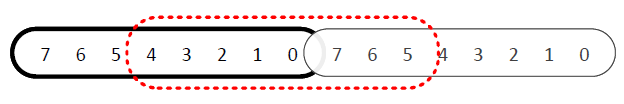
\includegraphics[scale=0.6]{Round_numbers.png}
% \caption{}
% \label{}
\end{figure}






